\chapter {Antecedentes}
\section {Sistemas de información geográfica}
  \paragraph {Un Sistema de Información Geográfica (GIS, por sus siglas en inglés) es un sistema computacional de captura, almacenamiento, chequeo y exposición de datos relacionados a la superficie de la Tierra. Los SIG pueden mostrar información de varios tipos en un mismo lienzo (usualmente mapas) lo que facilita el análisis de la información recolectada.\cite{5}}

  \paragraph{Los SIGs son una herramienta usada por organizaciones, escuelas, instituciones gubernamentales y negocios. Éstos sistemas pueden ser orientados a datos globales o a una región en específico del globo terraqueo. Entre los datos almacenados más importantes se encuentra la georeferenciación (Longitud, Latitud, Altitud), algunos datos relativos a la zona, por ejemplo, códigos postales.}

  \begin{figure}[h!]
      \centering
        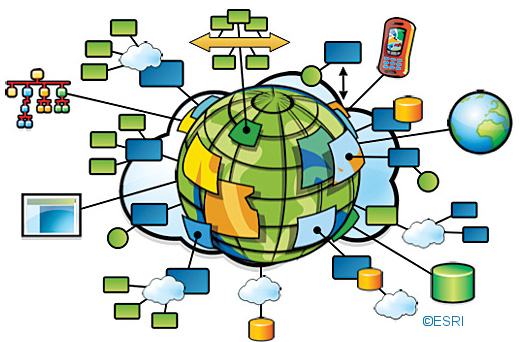
\includegraphics[width=\textwidth]{./images/GIS.jpg}
      \caption{Sistemas de Información Geográfica. \cite{18}}
  \end{figure}

  \paragraph{En México, la institución encargadada del manejo de datos estadíticos y geográficos es el INEGI. El Instituto Nacional de Estadística, Geografía e Informática (INEGI) es la fusión de varias instituciones gubernamentales que funcionaban de forma independiente hasta el año 1983; éstas se encargaban de el manejo de datos estadísticos, comerciales, económicos y financieros.}

  \paragraph{Actualmente el INEGI, sede se encuentra ubicada en Aguascalientes, Aguascalientes, es la institución encargada de la captación, procesamiento y difusión de información relativa al territorio nacional. \cite{6}}

  \paragraph{Los datos geoespaciales (Longitud, Latitud, Altitud) que brinda el INEGI se encuentran bajo el estandar \textbf{ITRF 2008} en época 2010. Sin embargo, aún existen sistemas que se encuentran trabajando bajo el formato ITRF92 época 1988 y NAD27 (formato usado hasta 1998), para ello, se brindará soporte a formatos previos, dando prioridad al último estandar existente.} 

\section {Sistemas de Monitoreo del medio Ambiente.}
  \subsection {Proyecto en la ciudad de Salamanca}
    \paragraph {Uno de los proyectos nacionales que realizo un monitoreo usando un PCFM fue realizado en la ciudad de Salamanca- una de las ciudades más contaminadas en México. Este proyecto es titulado “Análisis de la contaminación del aire usando un Algoritmo PCFM  aplicado a una base de datos real.}

    \paragraph{La intención del estudio es analizar la relación entre contaminación y las variables ambientales. En el análisis de este estudio se involucraron datos desde Enero a Diciembre del 2007. Algunas de las variables que se incluyeron fueron S02, y la concentración de partículas menores a 10m y variables meteorológicas. Velocidad del viendo, dirección del viento, temperatura y humedad relativa. A partir de este estudio se instalaron algunos centros de monitoreo en Salamanca.}

  \subsection {Inventario Nacional de Emisiones de Gases de Efecto Invernadero (INEGEI)}
    \paragraph {En este proyecto se elabora un informe que comprende las estimaciones de las emisiones por fuente y sumidero. Esto se realiza de acuerdo a lo conforme establecido en los artículos 4 y 12 de la Convención marco de las naciones unidas sobre el cambio climático. Este proyecto es una publicación que nos ayuda a saber que deficiencias tenemos, y que efectos pudiera llegar a tener el exceso de algunos contaminantes, sin embargo no es una plataforma para accede a estos datos tan importantes.}

  \subsection {Mapa Digital -  INEGI}
    \paragraph {Este proyecto es un sistema de información geográfica que tiene como objetivo facilitar el estudio de los objetos geográficos a través del conocimiento de su ubicación espacio-temporal, así como de atributos asociados;  tales servicios bridan al usuario final la posibilidad de:}

  \begin{itemize}
    \item {Mostrar en forma gráfica la dimensión de la información contenida por medio de acercamientos, selección de capas de información, localizaciones, mediciones, etc.}
    \item {Analizar e interpretar los contenidos geográficos y estadísticos mediante operaciones matemáticas, mapas temáticos, gráficos estadísticos, análisis espacial y estadísticos básicos.}
    \item {Integrar información a través de la incorporación de datos vectoriales y raster provenientes de archivos locales, conexiones a servicios WMS y base de datos geospaciales de PostGis.}
  \end{itemize}

  \paragraph{Toda la información que muestra el mapa digital del INEGI es obtenida por medio de servicios tipo REST, se puede hacer uso de éstos usando Web Scrapping, sin embargo, se encuentra totalmente ligado a la aplicación, trayendo consigo problemas en caso de que se deseara extraer el contenido que ofrecen.}

  \begin{figure}[h!]
      \centering
        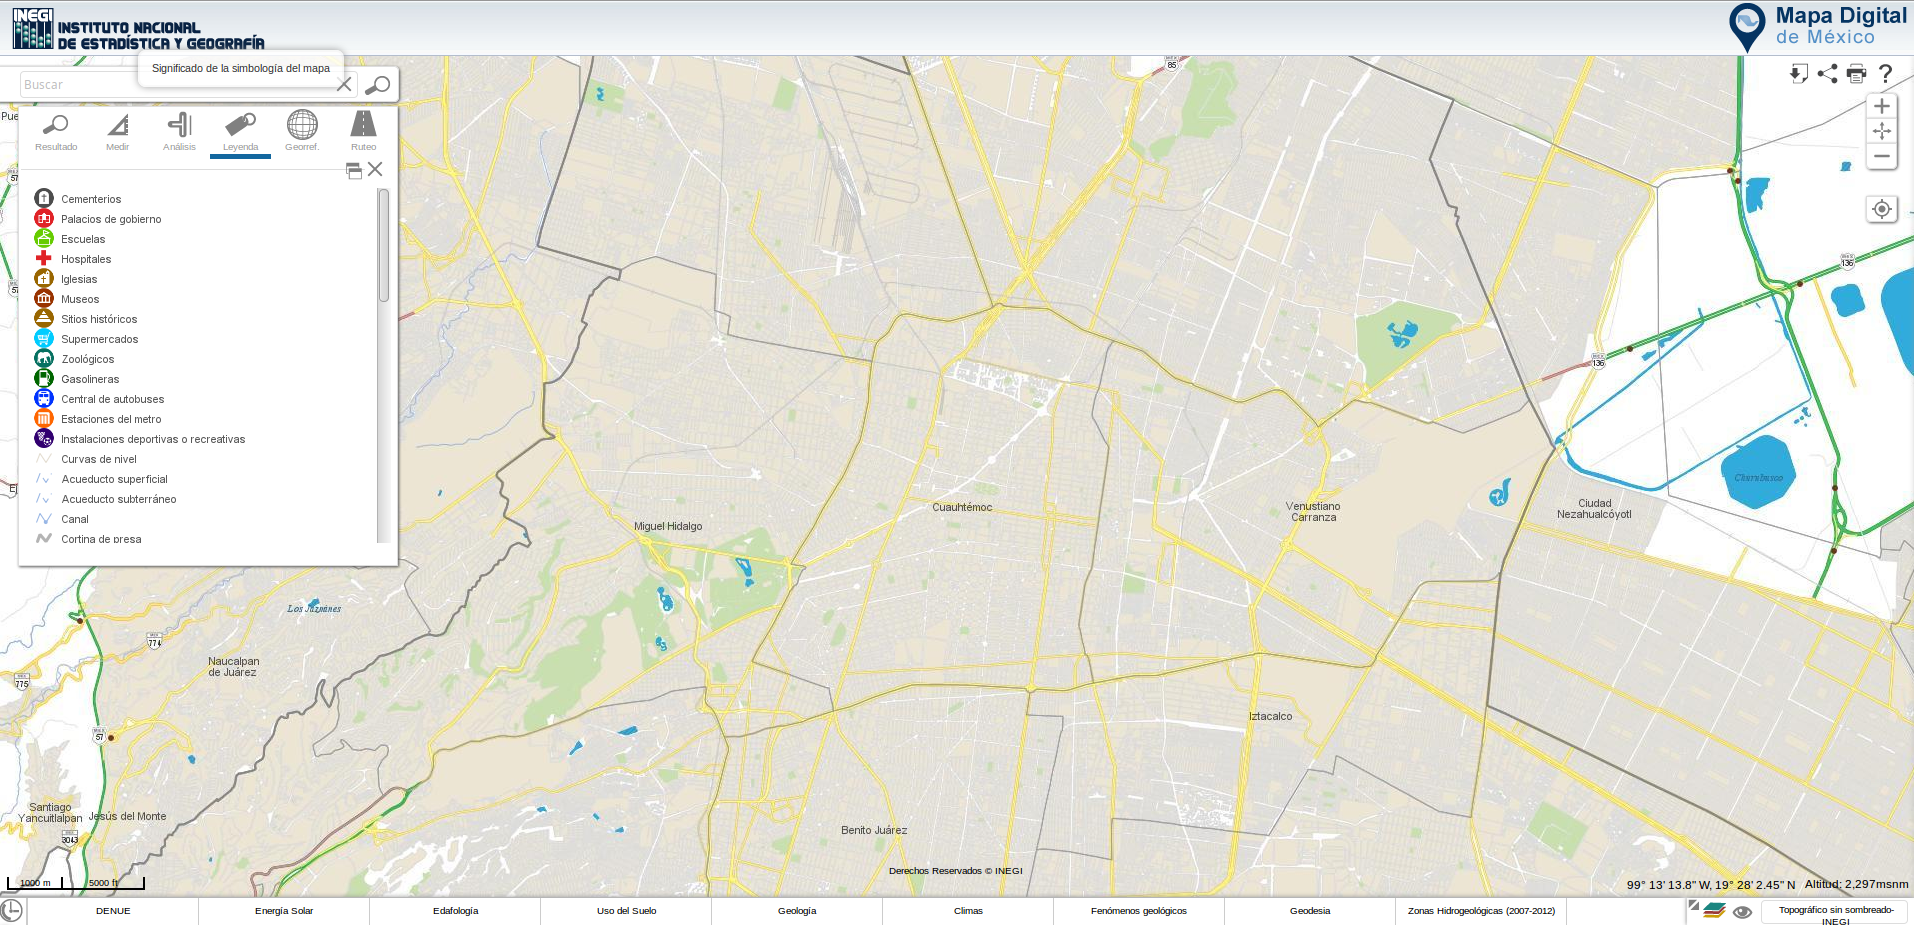
\includegraphics[width=\textwidth]{./images/MapaDigital.png}
      \caption{Mapa Digital - INEGI.}
  \end{figure}

  \paragraph{El INEGI y el mapa digital cuentan con algunos puntos de acceso a la información usando como medio principal las peticiones HTTP. Estos servicios suelen ser aislados y requieren de una interacción directa con el humano, es decir, es necesario que éste tenga una interacción mediante escritura o clicks en los formularios de éstos.}

  \subsection {Base de Datos Estadísticos BADESNIARN}
    \paragraph {Proyecto de la SEMARNAT que presenta información integrada, revisada y validada con cada una de las fuentes. Además esta estructurada para adecuarse a las necesidades de cada usuario . El usuario en su consulta encontrará el último dato revisado con la fuente, así como la serie histórica disponible en cada caso. Finalmente la plataforma tecnológica detrás le permitirá obtener un archivo electrónica en varios formatos con la info que muestra en pantalla.}    

    \paragraph { Tiene un módulo de consultas temática en donde están muy bien delimitados los temas relacionados con el ambiente, y uno dinámica en donde se asocia cada metadato o archivo con palabras clave para que el usuario pueda encontrar el tema de su interés. \cite{17}}

    \begin{figure}[h!]
        \centering
          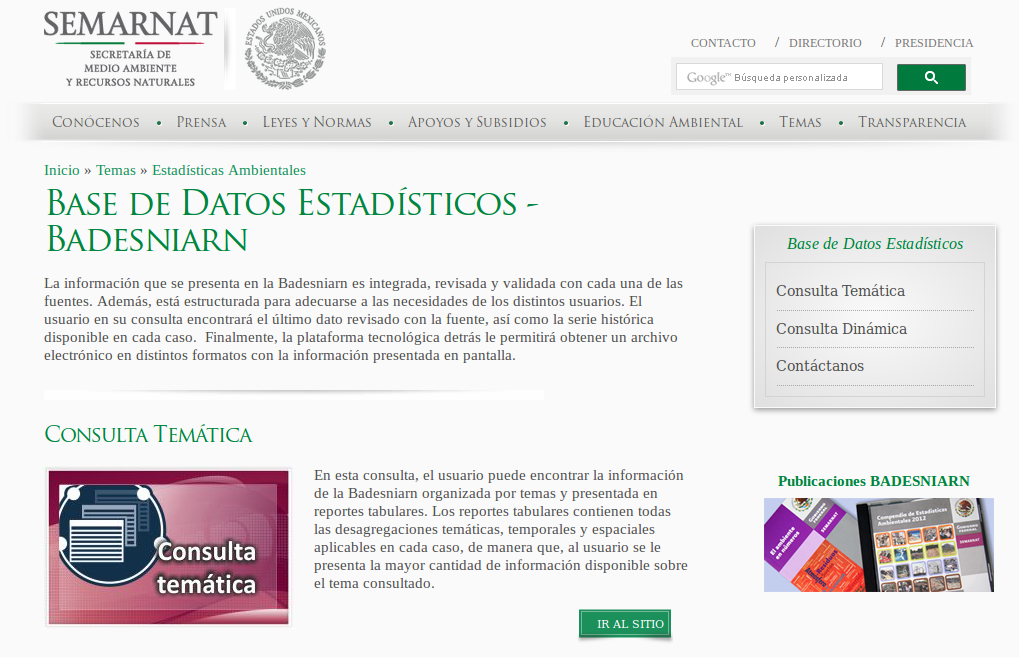
\includegraphics[width=\textwidth]{./images/BADESNIARN.png}
        \caption{Base de datos estadísticos - SEMARNAT.}
    \end{figure}

  \subsection {Forecast IO}
    \paragraph {Es un atlas del clima que se puede visualizar a través de una página web. En el se pueden consultar datos climatológicos – tales como la temperatura actual, probabilidades de precipitación considrando como modo de visualización base mapas de alta definición.}

    \paragraph{Este proyecto integra la información de diversas fuentes y también provee un servicio para obtener datos a través de peticiones REST. Una de sus más grandes desventajas es la limitante de peticiones hacia su servicio, ya que después de cierta cantidad se aplican cargos a una tarjeta definida al dar de alta la cuenta de desarrollador en la plataforma. \cite{14}}

    \begin{figure}[h!]
        \centering
          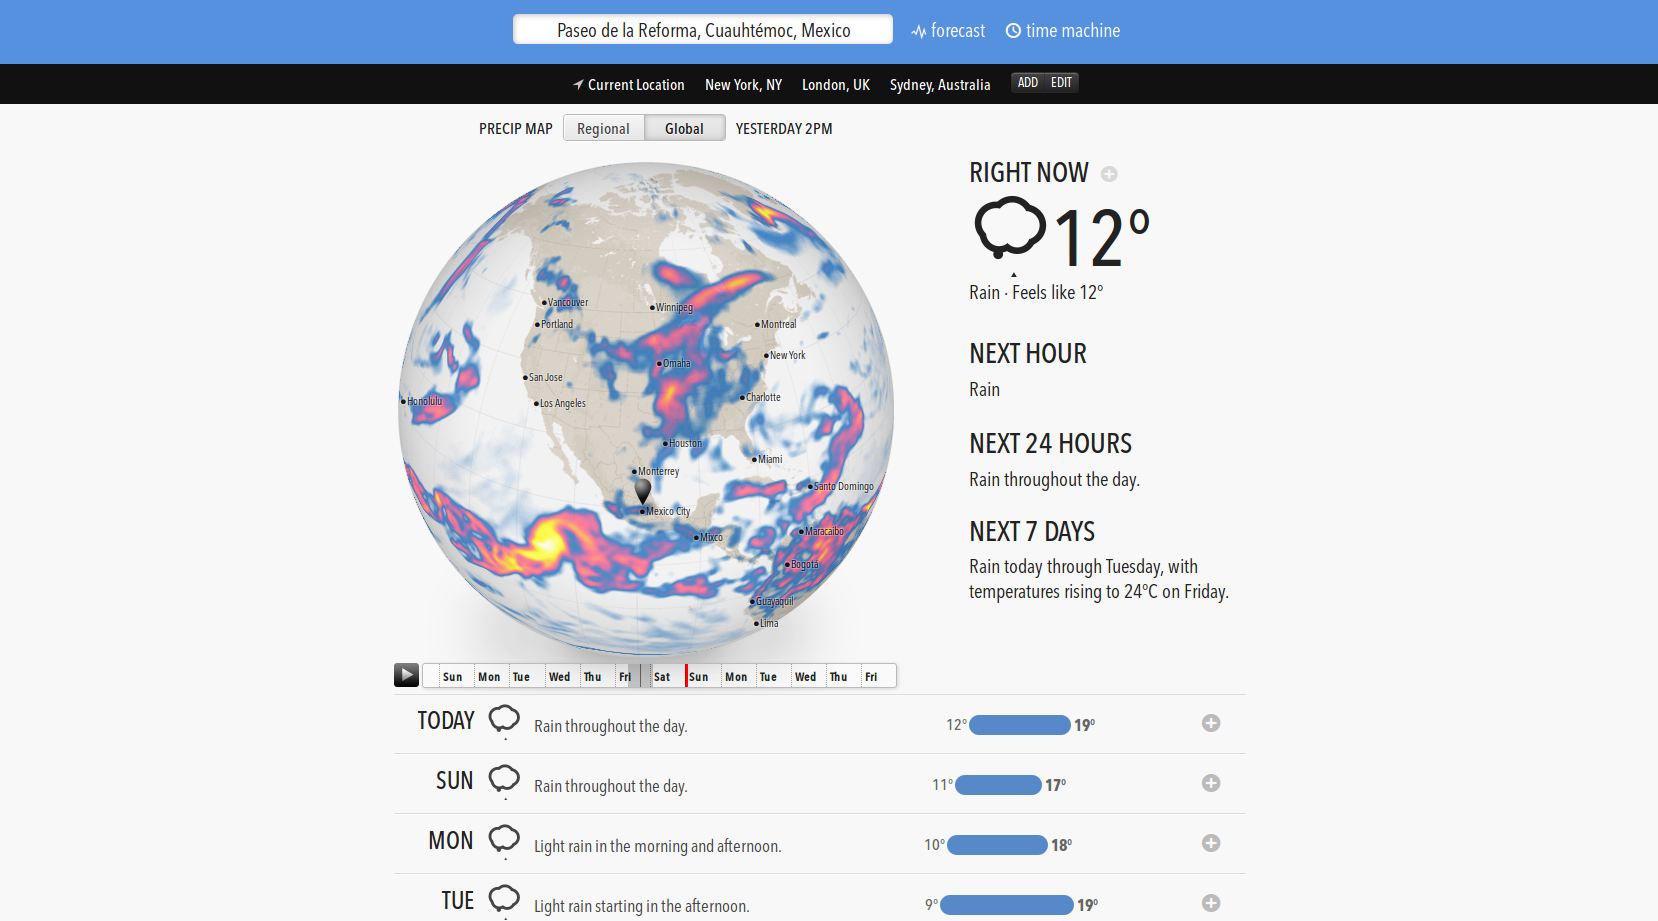
\includegraphics[width=\textwidth]{./images/ForecastIO.png}
        \caption{Forecast.io}
    \end{figure}    

\section{Sistemas de estandarización y unificación de datos.}
  \subsection{Proyecto INSPIRE.}
    \paragraph{El Proyecto INSPIRE comenzó a ser desarrollado el 15 de Mayo 2007 y será completamente implementado para el año 2019. Su principal objetivo es es la creación de una infraestructura única de información espacial a lo largo de la unión europea.} 
    \paragraph{La infraestructura de datos espaciales asistirá y trabajará a lo largo de todo el territorio Europeo y parte de Asia(Territorio de perteneciente a Rusia), los datos serán diversos considerando temás comunes y técnicos.}
    \paragraph{El proyecto INSPIRE trabaja bajo algunos principios, por ejemplo:}
    \begin{itemize}
      \item Los datos deben ser recabados sólo una vez y mantenerse actualizados de forma efectiva.
      \item Es posible combinar información espacial de varias fuentes a través del territorio Europeo y compartir sus aplicaciones.
      \item La información geográfica almacenada en todos los niveles será transparente y compartida.
      \item Busqueda fácil de de información geográfica que puede ser usada para fines particulares y de uso general.
    \end{itemize}
    \paragraph{Actualmente parte de los modulos desarrollados se encuentran en etapas de pruebas. Cuenta con un editor de metadatos }
  \subsection{Geoplatform}
    \paragraph{Plataforma propuesta por el gobierno de Estados Unidos, principalmente por el Comité Federal de Datos Geográficos (The Federal Geographic Data Committee) \cite{19}. Actualmente funciona como una PaaS (Platform as a Service), cuyos principales objetivos son:}
    \begin{itemize}
      \item {Unificar y brindar información geoespacial confiable a través de datos y servicios.}
      \item {Soporte para toma de decisiones.}
      \item{Aplicación para la solución de problemas que pueden ser desarrollados sólo una vez y usados varias veces a través de distintas instituciones federales y otras organizaciones.}
      \item{Infraestructura compartida para almacenar datos y aplicaciones.}
      \item{Punto focal donde instituciones gubernamentales, académicas, privadas y públicas pueden visualizar información relativa a su región.}
  \end{itemize}
  \paragraph{Actualmente usan un estándar de datos abierto conocido como “Common Core Metadata Schema” bajo su versión 1. \cite{20}}

  \begin{figure}[h!]
        \centering
          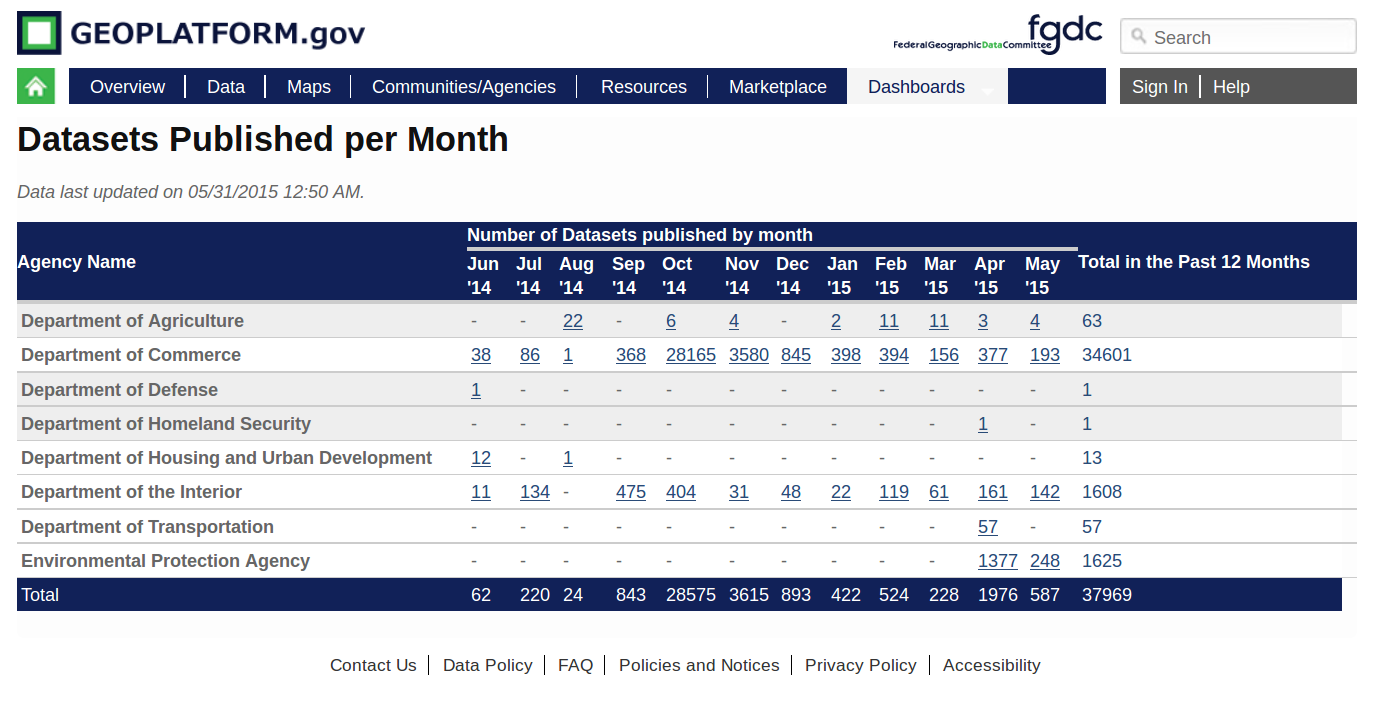
\includegraphics[width=\textwidth]{./images/GeoPlatform.png}
        \caption{Datasets publicados por Geoplatform}
    \end{figure}    

  \paragraph{La implementación de esta plataforma fue motivada por los principios y espirito de ``Open Government''\cite{21}, cuya principal visión es la de enfatizar la comunicación, contabilidad y transparencia entre gobierno-ciudadano, dentro del territorio estadounidense. Todos los datos, aplicaciones y servicios que provee Geoplatform se encuentran bajo licencias libres.}
  \paragraph{La plataforma fue desarrollada por miembros de la el comité federal de datos geográficos (FGDC por sus siglas en inglés) mediante la coolaboración de escuelas y usuarios expertos en el área. La audiencia que toma como fuente incluye agencias federales, estatales y locales, además de sector privado, educativo y al público en general. \cite{19}}
  \subsection{GeoMap México}
    \paragraph{}
\section{Características climáticas y de contaminación en México.}
  \subsection{¿Cuándo se iniciaron los problemas de contaminación del aire?}
    \paragraph {Desde siempre la humanidad ha emitido contaminantes al aire, pero esto se incrementó de manera dramática a partir de la Revolución Industrial iniciada en el Reino Unido a finales del siglo XVII. En esa época, el trabajo manual fue remplazado por maquinaria, básicamente por la introducción de tecnologías que empleaban el vapor y que hacían posible tener altos niveles de producción. El problema fue que con estos avances industriales se incrementó el  uso de combustibles, tal como el petróleo y el carbón mineral, ambos indispensables para el funcionamiento de la nueva maquinaria.}

    \paragraph {Desde entonces el problema de contaminación del aire se ha convertido en una constante en muchas ciudades industriales de todo el mundo, lo que ha ocasionado problemas de salud a su población.}

    \paragraph {Algunos de los casos más dramáticos y graves son la famosa niebla tóxica londinense de 1952, el deterioro de los bosques europeos por la lluvia ácida en los años cincuenta y sesenta del siglo XX, y la grave situación de la calidad del aire en la Ciudad de México, Tokio y Sao Paulo durante las últimas décadas del siglo anterior. }

  \subsection {¿Cuáles son los contaminantes y qué efectos tienen?}
    \paragraph {Los contaminantes pueden ser emitidos de forma natural o por actividades relacionadas con el ser humano. Los fenómenos naturales que se producen en la superficie o  en el interior de la tierra –como el caso de erupciones volcánicas, que produce emisiones de gases, vapores, polvos y aerosoloes-, también contribuyen a la contaminación del aire.}
    
    \paragraph {Los principales contaminantes relacionados con la calidad del aire son el bióxido de azufre (SO2), el monóxido de carbono (CO), los óxidos  de nitrógeno (NOx), las partículas suspendidas, el plomo y el ozono.}
  
    \begin{figure}[h!]
      \centering
       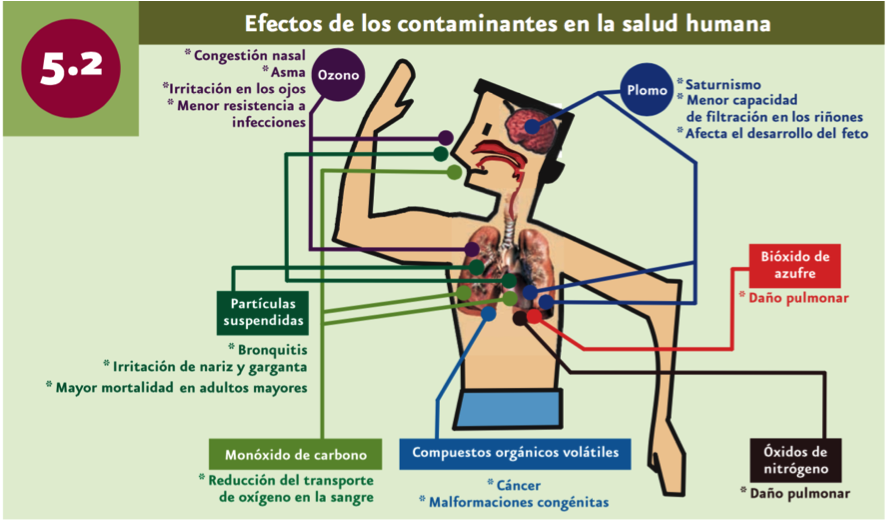
\includegraphics[width=12.5cm,height=9cm]{./images/1.png}
       \caption{Efectos de los contaminantes en el cuerpo.}
    \end{figure}

    \paragraph {Las plantas, animales y otros organismos también resienten los efectos de contaminantes como el ozono. Principalmente con la formación de la lluvia ácida, dicha lluvia es ocasionada con la presencia de ciertos ácidos en la atomósfera que se precipitan a la tierra con la lluvia. El dióxido de azufre y los óxidos de nitrógeno, resultado de la quema de combustibles  fósiles causan lluvia ácida, ya que al combinarse con agua, oxígeno y otros compuestos químicos forman ácidos como el ácido sulfúrico y el nítrico. }
    \paragraph{Las plantas se ven afectadas por esta lluvia ya que los ácidos pueden obstruir y acidificar los diminutos poros de las hojas por los que las plantas toman el aire que necesitan para realizar la fotosíntesis, además la lluvia ácida degrada los suelos, lo cual afecta las raíces y la nutrición de las plantas.}
  
    \paragraph {En el parque nacional Izta-Popo, Zoquiapan y en el Parque Nacional Desierto de los Leones, la lluvia ácida a dañado la vegetación. Estos daños involucran la pérdida de hojas y ramas, crecimiento lento y vulneravilidad a ataques de plagas y enfermedades.}
  
    \paragraph {Por otro lado los ríos, lagos y lagunas también pueden hacerse más ácidos por efecto de la lluvia ácida, lo cual pone en serio riesgo a las especies de plantas y animales que los habitan. Algunos ejemplos de estos daños se encuentran en los lagos del norte de Europa, en los que se ha reportado inclusio que han quedado sin ninguna forma de vida luego de la contaminación por lluvia ácida.}

    \begin{figure}[h!]
      \centering
        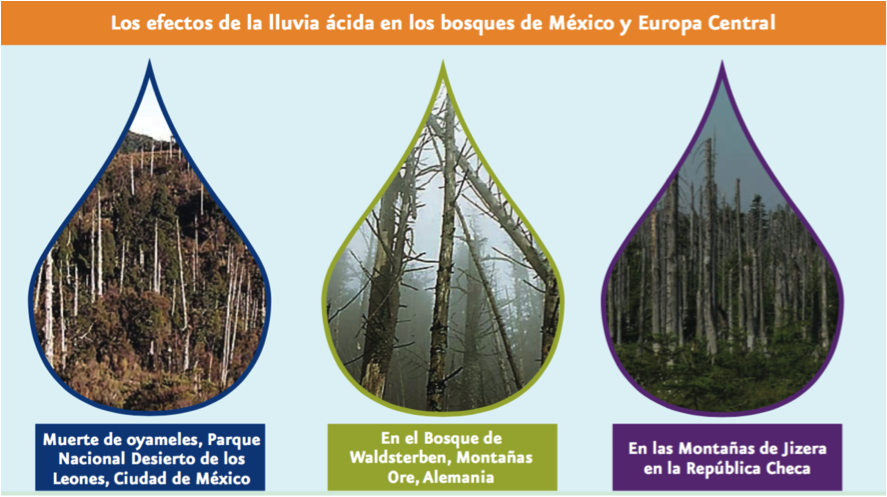
\includegraphics[width=\textwidth]{./images/2.png}      
      \caption{Impacto de la lluvia ácida en los bosques de México.}
    \end{figure}    

    \paragraph {Por otro lado también los monumentos y edificios sufren deterioros por la lluvia ácida, ya que los ácidos funcionan como agente corrosivo. El laboratorio de restauración del Instituto de Investigaciones Antropológicas de la UNAM indica que en losúltimos 25 años el deterioro de los monumentos y edificios históricos de la ciudad de México se ha acelerado de manera impresionante por el incremento de los niveles de contaminación.}

    \begin{figure}[h!]
      \centering
        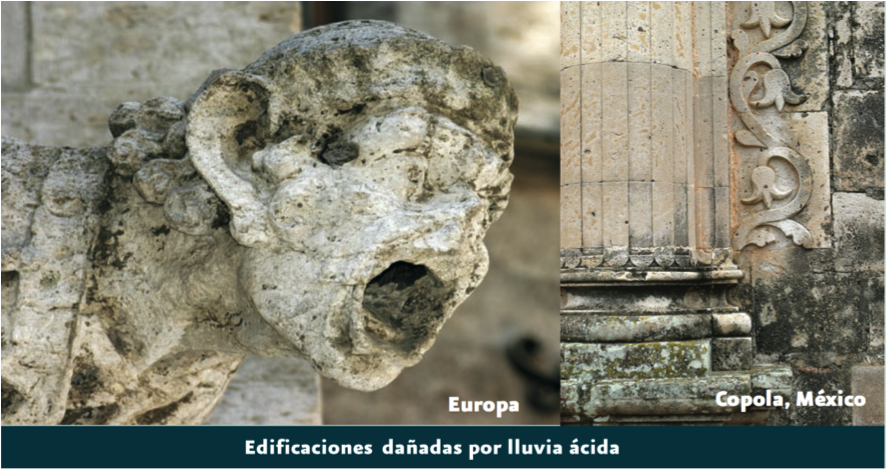
\includegraphics[width=\textwidth]{./images/3.png}
      \caption{Daños en edificaciones por lluvia ácida.}
    \end{figure}

  \subsection {Quiénes generan los contaminantes atmosféricos?}
    \paragraph {En México al igual que  en otros países se han desarrollado inventarios de emisiones que proporcionan información sobre la cantidad de contaminantes que se liberan al aire. En el año de 1999 de acuerdo al inventario de emisiones a nivel nacional se produjeron 40.5 millones de toneladas de las cuales el 58\% correspondieron a fuentes naturales- es decir, el suelo, la vegetación y las actividades volcánicas-    y 42\% a la contaminación de origen humano.}

    \paragraph {A pesar de que aparentemente las fuentes naturales sean las mayores productoras de contaminación, son las fuentes antropogénicas las que están cerca de la población y las que influyen en mayor medida en la calidad del aire que se respira.}

    \paragraph {Dentro de las fuentes antropogénicas, los vehículos automotores son los mayores productores de contaminantes, después la quema de gas LP y al final las emisiones de plantas generadoras de  electricidad.}

  \subsection {¿Qué hemos hecho para resolver el problema?}
    \paragraph {México lleva tiempo tomando acciones para resolver estos problemas, en 1988 implementó el Sistema Nacional del Inventario de Emisiones de Fuentes Fijas, así como un proyecto para cuantificar las emisiones del Valle de México. A partir del monitoreo de la calidad del aire ha diseñado algunas mejoras como eliminar el plomo en la gasolina, reducción del contenido de azufre.}

    \paragraph {Actualmente también existe una red de monitoreo atmosférico que abarca 52 ciudades y zonas metropolitanas que mide los niveles de contaminación presentes en el país. La concentración de los contaminantes en el aire se obtiene mediante la toma de muestras de aire que se analizan y procesan.}

    \paragraph {A partir de estas mediciones nacionales se han detectado cuales son las localidades con mayor índices de contaminación así como los contaminantes que emiten principalmente.  Uno de los esfuerzos más notables son los programas para mejorar la calidad del aire (Proaires) que buscan revertir las tendencias de deterioro, ya que incoroporan medidas para el control y abatimiento de las emisiones de los contaminantes.  También existen centrales eólicas para generar electricidad a partir de la energía del viento, una en la Venta, Oaxaca y la otra en Guerrero Negro, Baja California Sur.}